\documentclass{article}

\usepackage[utf8x]{inputenc}
\usepackage[english,russian]{babel}
\usepackage{cmap}
\usepackage{commath}
\usepackage{amsmath}
\usepackage{amsfonts}
\usepackage{mathtools}
\usepackage{amssymb}
\usepackage{parskip}
\usepackage{titling}
\usepackage{color}
\usepackage{hyperref}
\usepackage{cancel}
\usepackage{enumerate}
\usepackage{multicol}
\usepackage{graphicx}
\usepackage[font=small,labelfont=bf]{caption}
\usepackage[a4paper, left=2.5cm, right=1.5cm, top=2.5cm, bottom=2.5cm]{geometry}

\graphicspath{ {./images/} }
\setlength{\droptitle}{-3cm}
\hypersetup{ colorlinks=true, linktoc=all, linkcolor=blue }
\pagenumbering{arabic}

\begin{document}
\subsection{Возрастание и убывание функции на интервале и в точке. Локальный экстремум}

\textbf{Определение.} Функция называется строго возрастающей на интервале \((a, b)\)(или на промежутке \([a, b]\), если

\[\forall x_1, x_2 \in (a,b)([a,b]): x_1 < x_2 \Rightarrow f(x_1) < f(x_2)\]

\textbf{Определение.} Функция называется неубывающей на интервале \((a, b)\)(или на промежутке \([a, b]\)), если

\[\forall x_1, x_2 \in (a, b)([a, b]): x_1 < x_2 \Rightarrow f(x_1) \leq f(x_2)\]

Аналогично давали определение строго убывающей и невозрастающей на \((a, b)\)(или \([a,b]\)) функции.

Пусть теперь функция \(y = f(x)\) определена в некоторой окрестности точки \(x\). Для достаточно малых \(\Delta x\) имеет смысл \(\Delta y = f(x+\Delta x) - f(x)\) в точке \(x\).

\textbf{Определение.} Функция \(y = f(x)\)

\begin{enumerate}
    \item Возрастает в точке \(x\), если \(\exists \delta > 0\ \forall \Delta x: 0 < \abs{\Delta x} < \delta\ \frac{\Delta y}{\Delta x} = \frac{f(x+\Delta x)-f(x)}{\Delta x} > 0\)
    
    (\(\exists \delta > 0\ \forall x_1 \in (x-\delta, x), x_2 \in (x, x + \delta)\ f(x_1) < f(x) < f(x_2)\))
    \item Убывает в точке \(x\), если \(\exists \delta > 0\ \forall \Delta x: 0 < \abs{\Delta x} < \delta\ \frac{\Delta y}{\Delta x} = \frac{f(x+\Delta x)-f(x)}{\Delta x} < 0\)
    
    (\(\exists \delta > 0\ \forall x_1 \in (x-\delta, x), x_2 \in (x, x + \delta)\ f(x_1) > f(x) > f(x_2)\))
    \item Достигает локального максимума в точке \(x\), если
    
    \(\exists \delta > 0\ \forall \Delta x: \abs{\Delta x} < \delta\ \Delta y < 0(\exists \delta > 0\ \forall x_1 \in (x - \delta, x + \delta)\ f(x_1) < f(x))\)
    \item Достигает локального минимума в точке \(x\), если
    
    \(\exists \delta > 0\ \forall \Delta x: \abs{\Delta x} < \delta\ \Delta y > 0(\exists \delta > 0\ \forall x_1 \in (x - \delta, x + \delta)\ f(x_1) > f(x))\)
\end{enumerate}

\textbf{Замечание.} Здесь \(\Delta x\) малая величина как \(>0\), так и \(<0\), т.е. работаем с двусторонними окрестностями.

\textbf{Теорема.}(*) Если функция \(y = f(x)\) в точке \(x\) имеет положительную(отрицательную) производную, то она возрастает(убывает) в этой точке.

\(\uparrow\) Пусть \(f'(x) > 0\), т.е. \(\lim_{\Delta x \to 0} \frac{\Delta y}{\Delta x} = A > 0\).

По теореме об отделении от нуля для пределов функций получаем, что в окрестности т. \(x\ \exists \delta > 0:\ \forall \abs{\Delta x} < \delta\ \frac{\Delta y}{\Delta x} > 0\).

Таким образом, по п.1 определения \(y = f(x)\) возрастает в точке \(x\). Аналогично можно доказать, если \(f(x) < 0\), то функция убывает в точке \(x.\ \downarrow\)

\subsubsection{Теорема Ферма или необходимое условие экстремума}

\textbf{Теорема.} Если функция \(y = f(x)\) достигает в точке \(x\) локальный экстремум и в ней существует производная функции, то последняя равна нулю, т.е. \(f'(x) = 0\).

\(\uparrow\) Если \(f'(x) \neq 0\), то по (*) \(y = f(x)\) или возрастает, или убывает в этой точке, что исключает существование экстремума. Противоречие. \(\downarrow\)

\textbf{Замечания.}
\begin{enumerate}
    \item Теорема Ферма необходимое, но не достаточное условие существования экстремума в точке. \(y = x^3,\ y' = 3x^2 = 0 \Leftrightarrow x = 0\), но \(y = x^3\) возрастает в этой точке.
    \item Среди точек локального экстремума могут быть точки, где производная не существует: \(y = \abs{x}\).
\end{enumerate}

\textbf{Важный вывод:} Экстремумы исследуемой функции ищутся среди точек из О.О.: производная в этой точке \(= 0\) или не существует.

\subsection{Теоремы о среднем значении. Критерии возрастания и убывания функции на интервале. Достаточные условия существования локальных экстремумов}

\subsubsection{Теорема Ролля}

\textbf{Теорема.} Пусть функция \(y = f(x)\) непрерывна на отрезке \([a, b]\), имеет производную на интервале \((a, b)\) и принимает равные значения на концах отрезка, т.е. \(f(a) = f(b)\), тогда существует хотя бы одна точка \(c \in (a, b):\ f'(c) = 0\).

\(\uparrow\) Так как функция \(y = f(x)\) непрерывна на отрезке \([a, b]\), то по теореме Вейерштрасса она достигает на этом отрезке своего наибольшего(\(M = {max}_{[a, b]}f(x)\)) и наименьшего(\(m = {min}_{[a, b]}f(x)\)) значения.

Если \(m = M = f(a)\), то \(f(x) = M\), т.е. \(f(x) = const\), и \(f'(c) = 0\) в любой \(c \in (a, b)\).

Если \(m = M = f(a)\) не выполняется, то или \(f(a) \neq M\), или \(f(a) \neq m\).

Пусть \(f(a) \neq M\), тогда в качестве \(c \in (a, b)\) можем рассмотреть точку, в которой достигается наибольшее значение: \(M = {max}_{[a, b]} f(x) = f(c)\).

В этой точке достигается локальный максимум, существует производная(условие), значит, по теореме Ферма \(f'(c) = 0\).

Случай \(f(a) \neq m\) рассматривается аналогично. \(\downarrow\)

\subsubsection{Теорема Лагранжа}

\textbf{Теорема о конечных приращениях.} Пусть функция \(y = f(x)\) непрерывна на отрезке \([a, b]\) и имеет производную на интервале \((a, b)\), тогда существует хотя бы одна \(c \in (a, b):\ f'(c) = \frac{f(b)-f(a)}{b-a}\).

\(\uparrow\) Рассмотрим функцию \(F(x) = f(x) - f(a) - \frac{f(b) - f(a)}{b - a}(x-a)\).

Заметим, что \(F(x)\) непрерывна на \([a, b]\), как разность непрерывных функций, дифференцируема на \((a, b)\), как разность дифференцируемых.

\(\begin{array}{l}
    F(a) = f(a) - f(a) - \frac{f(b)-f(a)}{b-a}(a-a) = 0\\
    F(b) = f(b) - f(a) - \frac{f(b)-f(a)}{b-a}(b-a) = 0
\end{array}\)
т.е. \(F(a) = F(b)\)

Значит, по теореме Ролля \(\exists c \in (a, b):\ F'(c) = 0\)

\(F'(x) = f'(x) - 0 - \frac{f(b) - f(a)}{b - a} \Rightarrow F'(c) = f'(c) - \frac{f(b) - f(a)}{b - a} = 0\ \downarrow\)

\textbf{Замечания.}
\begin{enumerate}
    \item Геометрический смысл теоремы Лагранжа.
    
    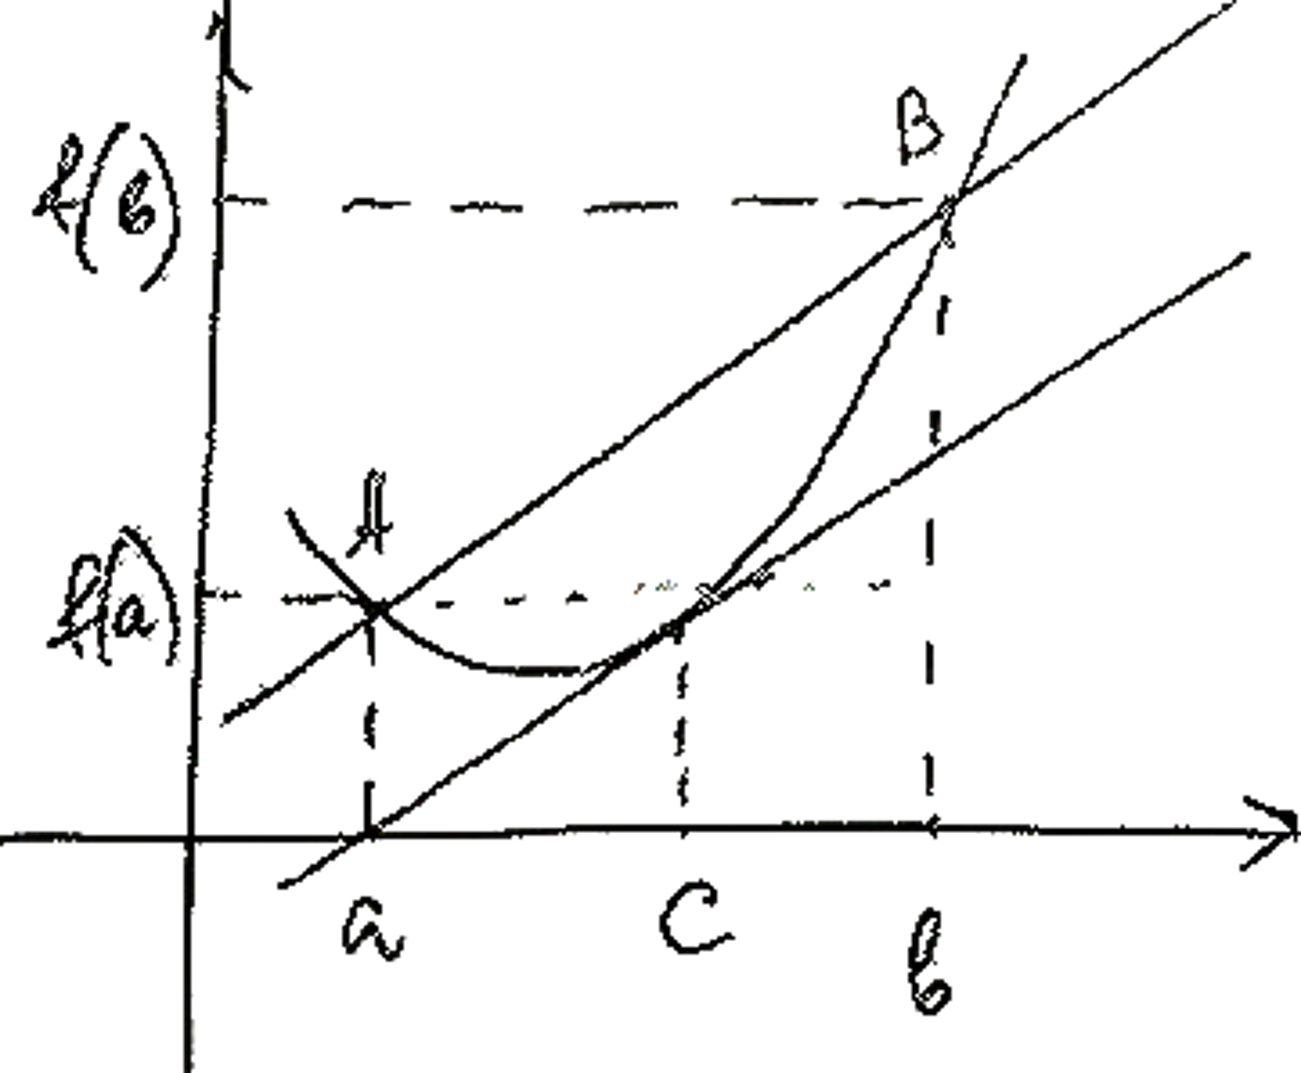
\includegraphics[scale=0.15]{11_1_10_1.png}
    \item Результат теоремы Лагранжа можно записать в вид \(f(b) - f(a) = f'(a + \Theta(b-a))(b-a),\ 0 < \Theta < 1\).
\end{enumerate}

\subsubsection{Теорема Коши}

\textbf{Теорема.} Пусть функции \(y = f(x)\) и \(y = g(x)\) непрерывны на отрезке \([a, b]\), имеют производные на интервале \((a, b)\), и \(g'(x) \neq 0\ (a,b)\), тогда существует хотя бы одна \(c \in (a,b):\ \frac{f(b) - f(a)}{g(b) - g(a)} = \frac{f'(c)}{g'(c)}\).

\(\uparrow\) Заметим, что \(g(b) \neq g(a)\). Если \(g(b) \neq g(a)\), то по теореме Ролля \(\exists\ c \in (a, b):\ g'(c) = 0\), что противоречит условию теоремы.

Рассмотрим вспомогательную функцию \(F(x) = f(x) - f(a) - \frac{f(b) - f(a)}{g(b) - g(a)}(g(x) - g(a))\).

Затем, что \(F(x)\) непрерывна на \([a, b]\), как разность непрерывных функций, дифференцируема на \((a, b)\), как разность дифференцируемых.

\(\begin{array}{l}
    F(a) = f(a) - f(a) - \frac{f(b)-f(a)}{g(b)-g(a)}(g(a)-g(a)) = 0\\
    F(b) = f(b) - f(a) - \frac{f(b)-f(a)}{g(b)-g(a)}(g(b)-g(a)) = 0
\end{array}\)
т.е. \(F(a) = F(b)\)

По теореме Ролля \(\exists c \in (a, b):\ f'(c) = 0\)

\(F'(x) = f'(x) - 0 - \frac{f(b) - f(a)}{g(b) - g(a)}g'(x) \Rightarrow F'(c) = f'(c) - \frac{f(b) - f(a)}{g(b) - g(a)}g'(c)=0\)

\subsubsection{Применения теорем о среднем}

\textbf{Теорема.} Функция, непрерывная на отрезке \([a, b]\) и имеющая производную \(f'(x) > 0(\geq 0)\) на интервале \((a, b)\), строго возрастает(не убывает) на \([a, b]\).

\(\uparrow\) Пусть \(x_1, x_2:\ a \leq x_1 < x_2 \leq b\), тогда на \([x_1, x_2]\) выполняются условия теоремы Лагранжа, следовательно, \(\exists c \in (x_1, x_2):\ f(x_2) - f(x_1) = f'(c) \cdot (x_2 - x_1)_{>0}\).

Если \(f'(x) > 0\), то \(f(x_2) - f(x_1) > 0\), т.е. функция строго возрастает на \([a, b]\),

Если \(f'(x) \geq 0\), то \(f(x_2) - f(x_1) \geq 0\), т.е. функция не убывает на \([a, b]\ \downarrow\)

\textbf{Теорема.} Если непрерывная на отрезке \([a, b]\) функция имеет на интервале \((a, b)\) производную, равную нулю, то эта функция постоянна на \([a, b]\).

\subsubsection{Теорема о первом достаточном критерии для существования локального экстремума}

\textbf{Теорема.} Если функция \(y=f(x)\) непрерывна в окрестности точки \(x_0\) и имеет производную в некоторой выколотой окрестности точки \(x_0\), то наличие локального экстремума определяется в соответсвии с таблицей:

\begin{tabular}{ | c | c | c | }
    \hline
    \(x \in \dot{U}(x_0):\ x < x_0\) & \(x \in \dot{U}(x_0):\ x > x_0\) & \(x_0\)\\ [4.5pt]\hline
    \(f'(x) < 0\) & \(f'(x) > 0\) & Точка локального минимума\\[4.5pt] \hline
    \(f'(x) > 0\) & \(f'(x) < 0\) & Точка локального максимума\\ [4.5pt]\hline
\end{tabular}

\(\uparrow\) из теоремы Лагранжа получали формулу конечных приращений. В окрестности точки \(x_0\) её можно записать:

\[\Delta f = f(x) - f(x_0) = f'(x_0 + \Theta(x-x_0)) \cdot (x-x_0),\ 0 < \Theta < 1\]

В 1м случае:
\begin{enumerate}
    \item Если \(x < x_0\) и \(f'(x) < 0\), то \(\Delta f > 0\)
    \item Если \(x > x_0\) и \(f'(x) > 0\), то \(\Delta f > 0\)
\end{enumerate}
\(\Delta f > 0\) в \(\dot{U}(x_0)\).

Аналогично 2й случай. \(\downarrow\)

\textbf{Замечание.} Обратите внимание, что в теореме не предполагалось существование \(f'(x_0)\).
\end{document}